\subsection{Verschachtelte Graphen}
%Hypernodes ermöglichen die Verschachtelung von Graphen, was bedeutet, dass ein Knoten wiederum ein Graph sein kann
In einem verschachtelten Graphen kann ein Knoten wiederum ein Graph sein. Diese Knoten werden als Hypernodes bezeichnet.
Das Konzept von Hypernodes erlaubt eine beliebig große Komplexität des Modells.
Das Hypernode Modell nutzt gerichtete Kanten.
Jeder Knoten des verschachtelten Graphen bekommt ein eindeutiges Label.
Um die Knoten in verschiedene Kategorien zu unterteilen werden Tags vergeben \cite{poulovassilis1994nested}.

Abbildung \ref{2.hypernode.image} stellt einen Teil des in \ref{2.property.image} dargestellten Property Graphen als Hypernodes dar.
Alle Knoten haben ein eindeutiges Label und es wurden zwei Tags vergeben - Unternehmen und Person.
Durch gerichtete Kanten werden die Beziehungen zwischen den einzelnen Hypernodes hergestellt.
Die Attributer, die im Property Graphen als Key-Value Paare gespeichert werden, werden im verschachtelten Graphen als Knoten einer Hypernode gespeichert.
\begin{figure}[H]
	\begin{center}
		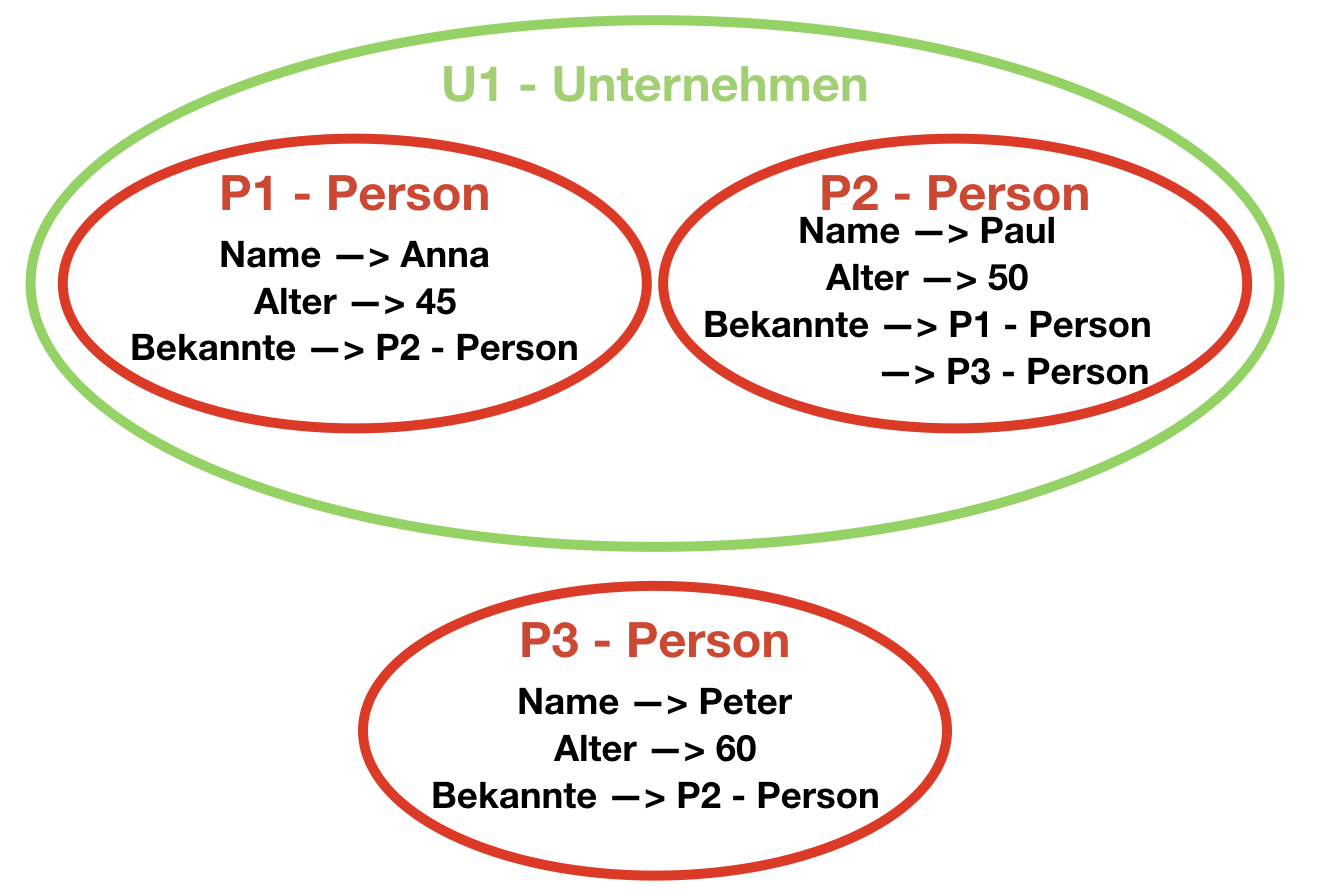
\includegraphics[scale = 0.5]{./images/Hypernode.png}
		\label{2.hypernode.image}
		\caption{Hypernode}
	\end{center}
\end{figure}

Hypergraphen lassen sich durch Hypernodes darstellen, indem man die im Hypergraph durch eine Hyperedge verbundenen Knoten in einer Hypernode modelliert.
Umgekehrt lassen sich Hypernodes nicht unbedingt in einem Hypergraphen realisieren \cite{poulovassilis1994nested}.